\documentclass[a4paper, 12pt]{scrartcl} 
\usepackage{ulem}
\usepackage{graphicx}
\usepackage{amsmath}
\usepackage[warn]{mathtext} 
\usepackage[T2A]{fontenc} 
\usepackage[utf8]{inputenc}
\usepackage[english]{babel} 
\usepackage{indentfirst} 
\usepackage{misccorr} 
\usepackage{caption}
\usepackage{graphicx}
\usepackage{subcaption}
\usepackage{xcolor}
\usepackage{wrapfig}
\usepackage{setspace}
\usepackage{algorithm}
\usepackage{algpseudocode}
\captionsetup{compatibility=false}
\begin{document}

\title{SyntenyFinder: A Synteny Blocks Generation and Genome Comparison Tool}
\author{Intern: Ilya Minkin\\
	Advisor: Son Pham}
\date{}
\maketitle
\algnotext{EndFor}
\algnotext{EndIf}
\algnotext{EndWhile}

\onehalfspacing

\begin{abstract}
    We present \textit{SyntenyFinder}, a de Bruijn graph based algorithm for finding synteny blocks in genomes. Our 
method is suitable for finding synteny blocks in genomes that contain regions of highly conserved DNA, i.e. genomes that are evolutionary
close to each other. We evaluated our tool on several datasets that include different strains of \textit{Mycobacterium tuberculosi} and 
\textit{Pseudomonas aeruginosa}. We also showed that with some modifications, the algorithm can be applied to generate synteny blocks in
distant genomes. 
\end{abstract}

\section{Introduction}

Recent advances in high throughput sequencing and genome assembling technologies are resulting in many 
finished genomes, ranging from bacterial to mammalian. The comparison of these genomes has been emerging as a powerful
tool for genome interpretations and has led to many important scientific discoveries.

The genome comparison tasks may be classified into two major directions: comparing genomes of different strains within the same species
and comparing genomes in different species. While comapring genomes from different species shines the light in their evolutional history, 
a finer look at the different and common regions of the closely related genomes (genomes within the same species) allows us to understand 
more about the function of many regions in these genomes and explains how these strains can adapt in different environments. 

%The genome comparison tasks often require to decompose the genomes into highly conserved sequence

%    It is known that genome rearrangements play important role in the evolution \cite{Pevzner2003a, Pevzner2003b, Bourque2004, Sankof2003}. The
%    rearrangements involve large portions of DNA and change their location and orientation. Particularly, rearrangements help bacteria in adaptation to various
%    environments \cite{Aujolat2012}. Another interesting evolutionary event is the whole genome duplication, which is usually
%    followed by massive gene loss \cite{Arabidopsis2000, Kellis2004}.

The genome comparison tasks often require genomes to be  decomposed to a collection of synteny blocks -- long regions of conserved DNA. Currently existing tools
\cite{Pham2010} are able to reconstruct synteny blocks from genomes represented as sequences of enumerated local alignments, or \textit{anchors}.
Usually, anchors denote homologous genes.

In this paper we propose \textit{SyntenyFinder} -- a tool for finding synteny blocks in genomes represented as nucleotide sequences.
Our approach is based on de Bruijn graphs that are extensively used in bioinformatics for genome assembly \cite{Pevzner2001, Iqbal2012}. 
It requires input genomes to share exact substrings of fixed length (\(> 100\) bp). Therefore, our method can be applied directly to only
closely related genomes, like different strains of the same species. But with some modifications it can be extended to wider range of use, i.e., 
finding synteny blocks in distant genomes.

In \textit{Overview} section we describe the problem definition and basic intuitions behind our method, section \textit{Algorithm Description}
contains formal description of our method. Finally, in \textit{Results} section, we benchmark our program on bacteria and yeasts datasets.

\section{Overview}

Given a set \(S = \lbrace S_{1}, S_{2}, \ldots, S_{n} \rbrace \) of chromosomes, where each
chromosome is represented as a string over alphabet \(\lbrace A, C, G, T \rbrace \). The task of finding synteny
blocks is to find a set of so called conserved regions \(C = \lbrace C_{1}, C_{2}, \ldots , C_{n} \rbrace \), where
each conserved region \(C_{i}\) is a set of substrings of chromosomes from \(S\). Such regions are supposed 
to cover most of the genome for closely related species.  All substrings forming a conserved region \(C_{i}\) must be
\textit{similar} to each other according to some criterion of similarity. Note that problem of finding synteny blocks in a set
of chromosomes is equivalent to a problem of finding synteny blocks in one superchromosome
obtained from concatenating all chromosomes from the set -- we can just separate chromosomes by special characters.

At this moment there is no generally accepted formal criterion of similarity exist, so the problem of finding synteny blocks is ill-defined.
In our work we introduce new criterion of similarity based on de Bruijn graphs and graph simplifications.

\begin{figure}
        \begin{subfigure}[a]{1\textwidth}
		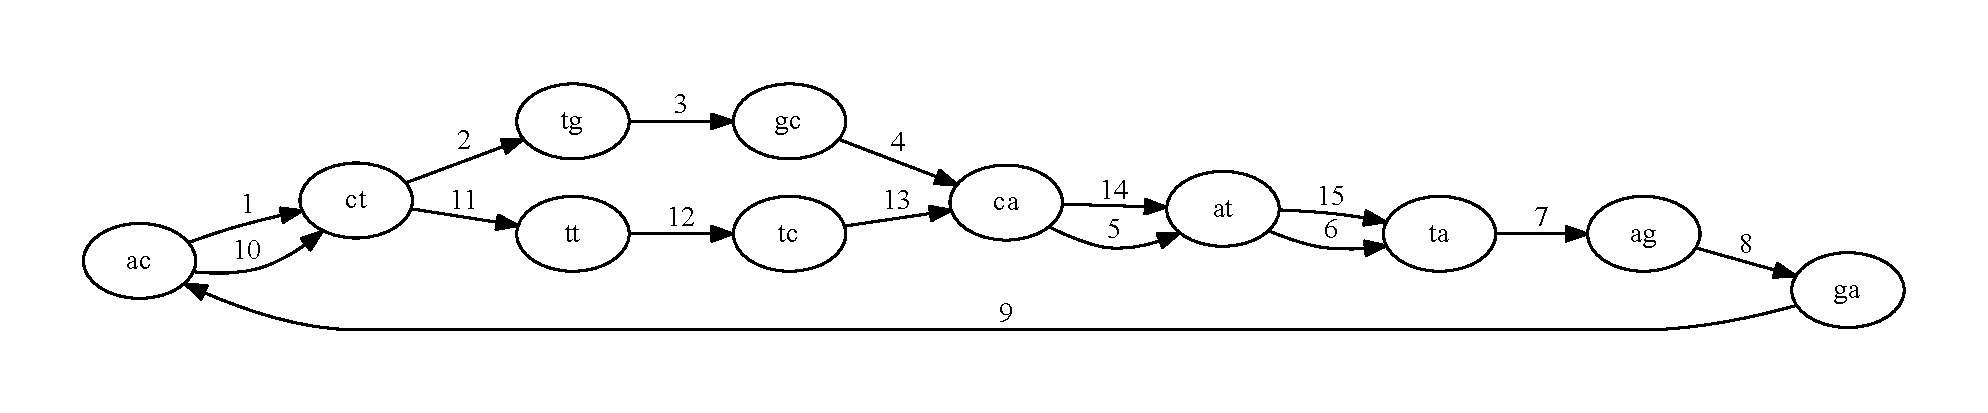
\includegraphics[scale = 0.45]{graph1.pdf}
		\small \caption{De Bruijn graph built from string \("actgcatagacttcata"\) and \(k = 2\). Non-branching paths correspond to multiple
			copies of the same substrings.}
		\label{DeBruijnA}
        \end{subfigure}
	\\
        \begin{subfigure}[b]{1\textwidth}
		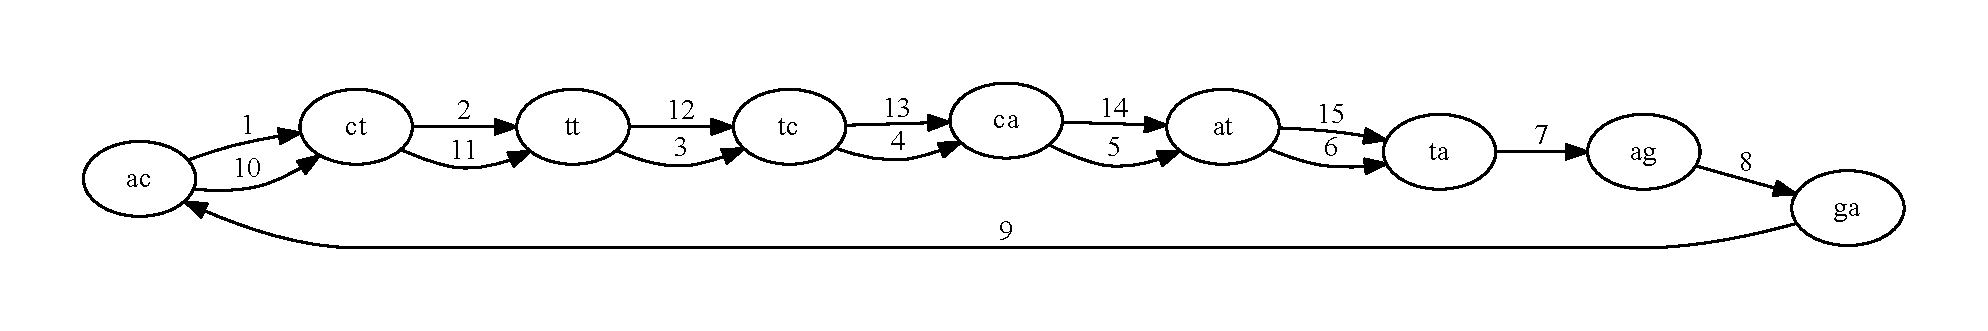
\includegraphics[scale = 0.45]{graph2.pdf}
		\small \caption{Same de Bruijn graph after simplification. Replacing substring \("ctGca"\) by \("ctTca"\) we obtain long non-branching path
			that corresponds to original synteny block.}
		\label{DeBruijnB}
        \end{subfigure}
	\small \caption{Illustration of de Bruijn graphs and graph simplification}
\end{figure}

As previously mentioned, our method is based on de Bruijn graph.
Given a fixed value \(k\) and a string \(S\) we can build de Bruijn graph \(G\) from the string as follows.
Let's denote by \(k\)-prefix of a string \(S\) the first \(k\) characters of \(S\), and by \(k\)-suffix the last \(k\) characters of \(S\).
For each unique substring of length \(k\) (called \(k\)-mer) found in \(S\), we add a vertex to \(G\) and mark it with
corresponding \(k\)-mer. For each \((k + 1)\)-mer \(w\) found in \(S\) we add edge that connects vertex corresponding to
\(k\) prefix of \(w\) with vertex corresponding to \(k\) suffix of \(w\) and label the edge with position of first character of \(w\)
(multiedges with different labels are allowed).

In this graph we consider only paths that have consecutive (that differ by 1) labels on edges. It is easy to see that with such restriction every path in \(G\)
corresponds to a substring in \(S\). Example of such de Bruijn graph built from the string \(S = "actgcatagacttcata" \) and \(k = 2\) is
depicted on Figure~\ref{DeBruijnA}.

Note that two copies of substring \("catt"\) form a non-branching path consisting of edges with multiplicity \(2\) in this graph. Single
mismatch in substrings \("ctGca"\) and \("ctTca"\) form so-called "bulge", unoriented cycle generated by two valid paths with
coinciding ends. If we replace one branch of the bulge by another (replace\("ctGca"\) by \("ctTca"\)), we obtain
a long non-branching path (Figure~\ref{DeBruijnB}).

This heuristic forms basis of our method -- conserved regions in different parts of the genome are usually 
disrupted by indels and mismatches. These differences form bulges in the graph that make it different to infer
structure of the synteny blocks. We remove bulges having size less than some predefined constant and thus obtain non-branching
paths corresponding to the conserved regions. The process of removing bulges from the graph is called \textit{simplification}. We
sustain one-to-one correspondence between the graph and the string -- when we change something in the graph, we also change
appropriate characters in the string.

Conserved regions can be located on opposite strands of DNA. To handle this, we add edges that correspond to reverse complementary
of the input string. We distinguish between direct and reverse complementary edges by coloring them in different colors.
Given a string \(S\), for each \((k + 1)\)-mer found in \(S\) we add corresponding edge to the graph and color it \textit{blue}, for 
each \((k + 1)\)-mer found in reverse-complementary counterpart of \(S\) we add corresponding edge to the graph and color it \textit{red}.
In this graph, non-branching paths with different colors represent synteny blocks located on opposite strands of DNA. The program 
consists of 4 steps:
\begin{itemize}
    \item Concatenate input chromosomes into one superchromosome 
    \item Build de Bruijn graph from the superchromosome 
    \item Simplify the graph 
    \item Output synteny blocks as non-branching paths in the graph 
\end{itemize}

Our algorithm depends on two parameters: \(k\) (vertices size) and \(\delta\) (minimum allowed size of a bulge). It is reasonable to use as high \(k\) as possible
\((k > 100)\) to keep graph structure simple and avoid connecting regions that are actually not homologous. So, our method requires that conserved regions
in input genomes contain exact shared \(k\)-mers. This is not a problem in genomes that are very close to each other (like different strains of a bacteria),
but it can create difficulties in genomes that have long evolutionary distances. 

This issue can be solved, for example, by finding a set of all local alignments in the genomes and substituting one subsequence in each found alignment
by another. In results section we will demonstrate on a practical half-synthetic example that with such modifications our method is able to handle
complicated cases. So at this point our method is directly applicable to only evolutionary close genomes and  in near future we plan to extend it to
wider range of use.

\section{Algorithm description}

Given two numbers \(k\) and \(\delta\) and a set \(S = \lbrace S_{1}, S_{2}, \ldots, S_{n} \rbrace \) of chromosomes,
where each chromosome  \(S_{i} = (s_{i, 1}, s_{i, 2}, \ldots, s_{i, m_i})\) is a string over alphabet \(\Sigma = \lbrace A, C, G, T \rbrace\).
Let's denote by \(X_{1} \uplus X_{2}\) concatenation of strings \(X_{1}\) and \(X_{2}\). We denote by \(X[i, j]\) a substring of a string \(X\) that
starts at \(i\) and ends at \(j\), \(X[i, j] = (x_{i}, x_{i + 1}, \ldots, x_{j}) \). \(Rev(X)\) means reverse-complementary counterpart of a string \(X\).

First step of the algorithm is to obtain superchromosome \(\hat{S} = S_{1} \uplus S_{2} \uplus \ldots \uplus S_{n} \). Concatenated
strings are interleaved by special characters that indicate ends of the chromosomes (we omit these technical details for simplicity of the description). 
We build a linked list of
pairs \(L = ((\hat{s}_1, 1), (\hat{s}_2, 2), \ldots, (\hat{s}_{m}, m))\) and \(l_i\) is a pointer to \(i\)-th item in the list, function \(Next(l_i) = l_{i + 1}\) returns
element after \(l_i\) in the list.
%Let's denote by \(l_i[1]\) the first element of pair of \(i\)-th item of the list (\(l_i[2]\) is the second element).
First element of a pair represents character of the sequence, and second element represents it's original position in string \(\hat{S}\). We preserve
original indices of the characters to be able to compute coordinates of the synteny blocks after graph simplification.
\(Ptr(L) = \) is a set of all pointers of a list \(L\). \( \mathcal P \left({Ptr(L)}\right) \) is a set of all subsets of \(Ptr(L)\).

Colored de Bruijn graph is graph \(G = (V, E) \) where \(V = \Sigma ^ k \). Set of outgoing edges from vertex \(v\) is denoted by \(Out(v)\). We define four functions: \\
1) \(Pos : \, E \rightarrow Ptr(L) \) \\
2) \(Color : \, E \rightarrow \lbrace Blue, Red \rbrace \) \\
3) \(Spell: \, E \rightarrow \Sigma ^ {k + 1} \) \\
4) \(Cover: \, E \rightarrow  \mathcal P \left({Ptr(L)}\right) \)

For each \(i \in \lbrace{1, 2, \ldots, n - k} \rbrace \) we add two oriented edges to the graph: \\
1) \(e^+ = (\hat{S}[i, i + k - 1], \hat{S}[i + 1, i + k]) \), where: \\
\(Pos(e^+) = l_i \\
Color(e^+) = Blue \\
Spell(e^+) = \hat{S}[i, i + k] \\
Cover(e^+) =  \lbrace l_i, l_{i + 1}, \ldots, l_{i + k} \rbrace \) \\
2) \(e^- = (Rev(\hat{S}[i, i + k - 1]), Rev(\hat{S}[i + 1, i + k]))\), where: \\
\(Pos(e^-) = l_{i + k} \\
Color(e^-) = Red \\
Spell(e^-) = Rev(\hat{S}[i, i + k]) \\
Cover(e^-) =  \lbrace l_i, l_{i + 1}, \ldots, l_{i + k} \rbrace \)

A \textit{valid} path in \(G\) is a sequence of edges \(P = (e_{1}, e_{2}, \ldots, e_{n})\) iff \(Pos(e_{i+1})  = Next(Pos(e_{i}))\) and
\(Color(e_{i + 1}) = Color(e_{i})\). Let's denote by \(Start(P)\) the first vertex of the path \(P\) and by \(End(P)\) the last vertex of \(P\).

A pair of valid paths \(B =\lbrace b_{1}, b_{2} \rbrace \)
is called a \textit{bulge}, iff following holds: \\
1) \(Start(b_{1}) = Start(b_{2}) \wedge End(b_{1}) = End(b_{2}) \) \\
2) There are no edges \(e_{1} \in b_{1}, e_{2} \in b_{2} \) such that \(Spell(e_{1}) = Spell(e_{2})\) \\
3) There are no edges \(e_{1} \in b_{1}, e_{2} \in b_{2} \) such that \(Cover(e_{1}) \cap Cover(e_{2}) \neq \emptyset\)

A bulge \(B =\lbrace b_{1}, b_{2} \rbrace \) is called \textit{bad} iff \(|b_1| < \delta \wedge |b_2| < \delta\) where \(\delta\) is a parameter.
A vertex \(v\) is called \textit{bifurcation} iff there are at least two outgoing (ingoing) edges \(e_{1}, e_{2}\) 
incident \(v\) such that \(Spell(e_{1}) \neq Spell(e_{2})\). Function \(MaxBifDegree(p)\) returns highest degree of a bifurcation that lies
on the path \(p\).

A set of paths \(P_{nb} = \lbrace P_{1}, P_{2}, \ldots, P_{n} \rbrace\)
is said to form a \textit{non-branching path} iff \(|P_{1}| = |P_{2}| = \ldots |P_{n}| \) and \(Spell(e_{i, k}) = Spell(e_{j, k}) \),
where \(e_{i, j}\) denote \(j\)-th edge in the \(i\)-th path, i.e. all paths spell the same substring.

\begin{figure}
	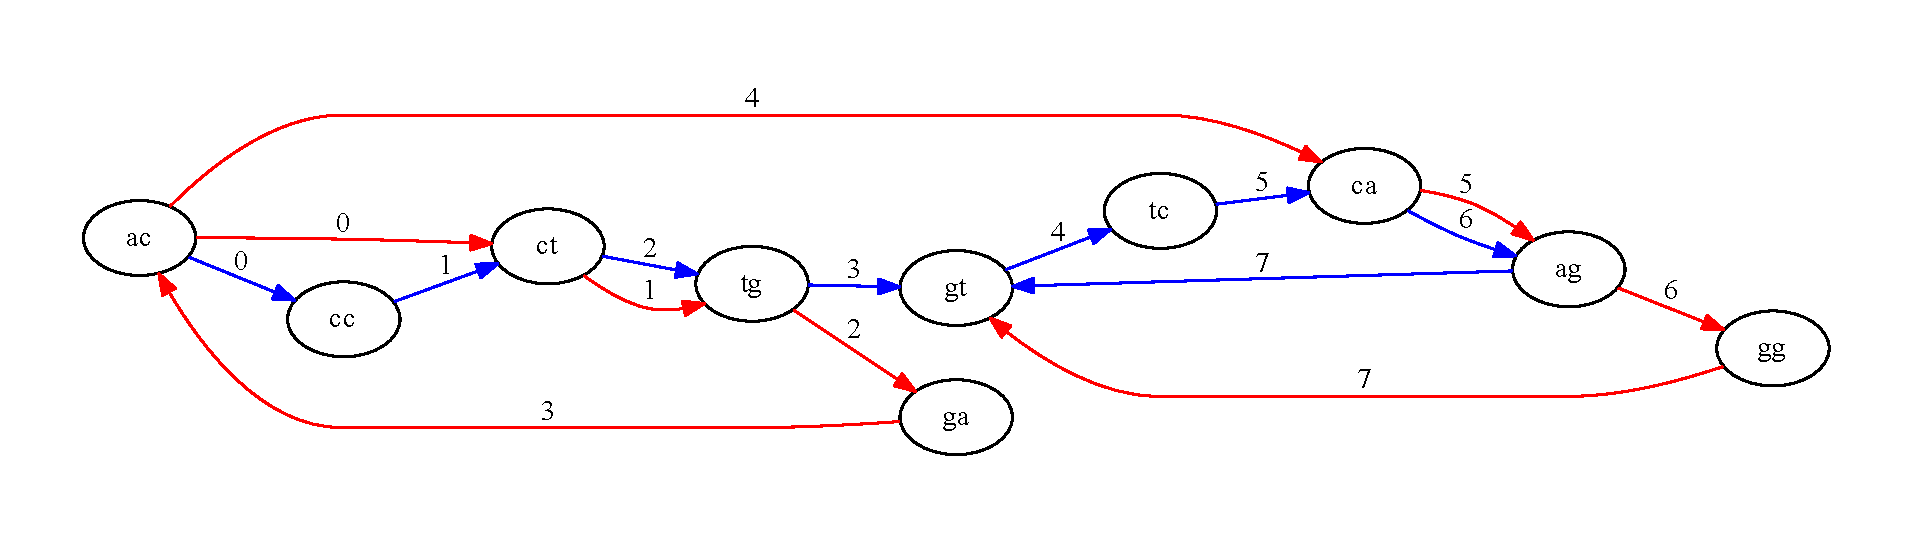
\includegraphics[scale = 0.50]{graph3.pdf}
	\small \caption{Colored de Bruijn graph for string \(S = "acctgtcagt" \) }
	\label{ColoredDeBruijn}
\end{figure}

Let's illustrate above definitions on a simple example. Colored de Bruijn graph built from string \(\hat{S} = "acctgtcagt"\)
is depicted on figure~\ref{ColoredDeBruijn}. Here \(Rev(\hat{S}) = "actgacaggt"\). Edges' labels denote indices of elements of
list \(L\). Vertices \("ac", "ct", "tg"\) are bifurcations, while \("cc", "tc", "ga"\) are not. Two paths \(("ac", "ct")\) and \((("ac", "cc"), ("cc", "ct"))\)
form a bulge. Two multiedges \(("ct", "tg")\) form a non-branching path.

Pseudocode of our algorithm for synteny blocks finding is presented below. Procedure of building a de Bruijn graph is described at the start of the section.
Function \(ProbeBadBulge(e_1, e_2,  \delta)\) trivially extends paths starting from edges \(e_1\) and \(e_2\) until they form a bad bulge or the branch length
threshold gets exceeded. It returns set of two paths if bad bulge was found and an empty set otherwise.
Procedure \(CollapseBadBulge(b_1, b_2, L, G)\) modifies the list \(L\) so that in the graph \(G\) path \(b_2\) gets replaced by path \(b_1\). 
Note that at any moment there is one-to-one correspondence between the list and the graph -- any changes in \(L\) are immediately reflected in \(G\).
Procedure \(OutputNonBranchingPaths(G)\) finds and outputs all maximal unique non-branching paths in \(G\)
and calculates starting and ending indices of the substring of the string \(\hat{S}\) that these paths correspond.

\begin{algorithm}[H]               
\small \caption*{\(SyntenyFinder(S = \lbrace S_{1}, S_{2}, \ldots, S_{n} \rbrace,  k, \delta)\)} 
\label{Pseudocode}
\begin{algorithmic}[1]     
\State \(\hat{S} = S_{1} \uplus S_{2} \uplus \ldots \uplus S_{n} \)
\State \(L = ((\hat{s}_1, 1), (\hat{s}_2, 2), \ldots, (\hat{s}_{m}, m))\)
\State \(G = BuildDeBruijnGraph(L, k)\)
\State \(run = True\)
\While{\(run == True\)}
	\State \(run = False\)
	\For{\(v \in V(G)\)}
		\For{\(e_1, e_2 \in Out(v)\)}
			\State \(\lbrace b_1, b_2 \rbrace = ProbeBadBulge(e_1, e_2,  \delta) \)
			\If{\(b_1 \neq \emptyset \, and \, b_2 \neq \emptyset \)}
				\State \(run = True\)
				\If{\(MaxBifDegree(b_1) > MaxBifDegree(b_2)\)}
					\State \(CollapseBadBulge(b_1, b_2, L, G)\)
				\Else	
					\State \(CollapseBadBulge(b_2, b_1, L, G)\)
				\EndIf
			\EndIf
		\EndFor
	\EndFor
\EndWhile
\State \(OutputNonBranchingPaths(G)\)
\end{algorithmic}
\end{algorithm}

\section{Experimental results}
We have implemented \textit{SyntenyFinder} in C++. To evaluate performance of our program, we benchmarked it on bacteria and yeasts datasets.

First dataset includes three strains of \textit{Mycobacterium tuberculosis} H37Rv: laboratory reference strain H37Rv,
CCDC5180, CCDC5079. We used \(K = 1000\) and \(\delta = 5000\) as parameters for this running. Our tool found
19 synteny blocks shared between all three genomes. These blocks cover 96\% of the genome.

Second dataset includes three strains of \textit{Pseudomonas aeruginosa}: 39016, UCBPP-PA14, PAO1 and NCGM2.S1.
Parameters were \(K = 1000\) and \(\delta = 5000\) as in previous test. We tool found 140 synteny blocks shared between four genomes. 
These blocks cover 90\% of the genome.

We also performed evaluation on well known yeast dataset including \textit{K.waltii} and \textit{S. cerevisiae}. Paper \cite{Kellis2004} describes
\(253\) so called regions of \textit{double conserved synteny}: DNA that are conserved between two regions in \textit{S. cerevisiae} and one region in \textit{K.waltii}.
Our method cannot be applied directly for this dataset since homologous genes in these genomes lack exact shared \(k\)-mers even for \(k < 20\). We used
matching of genes between these two genomes to enrich number of shared \(k\)-mers -- for each pair of homologous genes we substituted sequence of one
gene by another in the genome. We ran our program on the resulting enriched genome with \(k = 1000\) and \(\delta = 20 \,000\) and selected blocks shared
across all three genomes having size at least \(1 000\) base pairs. We have found \(270\) such blocks and \(185\) of them match the blocks described in \cite{Kellis2004}.
Total length of the blocks (we count only \textit{S. cerevisiae} regions) described in \cite{Kellis2004} is \(8  \, 390  \, 452\) bp, total length of our blocks is \(7 \, 773 \, 519\) bp, and \(6 \, 641 \, 468\) bp
from our blocks overlap with blocks from \cite{Kellis2004}. Our blocks cover  \(\frac{7 \, 773 \, 519}{12 \, 495 \, 682} \times 100 \% = 62\% \) of \textit{S. cerevisiae} genome. Most
blocks from \cite{Kellis2004} that are unmatched by our blocks are short (less than \(10 \, 000\) bp), many of them do not appear to be
synteny blocks when we manually check them. This half-synthetic example shows that
our method is indeed correct and after incorporating a local alignment tool our algorithm can be used to find synteny blocks even in complicated cases.


\section{Conclusion}
In this work we present an algorithm, that is able to find synteny blocks from unannotated sequences. It can be applied to genomes of species that are 
evolutionary close to each other.
With some modifications our method can be extended for finding synteny blocks in more distant genomes.


\begin{thebibliography}{99}
\bibitem{Pevzner2003a}
	Pavel Pevzner, Glenn Tesler.
	Genome rearrangements in mammalian evolution: lessons from human and mouse genomes.
	Genome Res. 2003 January 1; 13(1): 37–45.
\bibitem{Pevzner2003b}
	Pavel Pevzner, Glenn Tesler.
	Human and mouse genomic sequences reveal extensive breakpoint reuse in mammalian evolution
	PNAS June 24, 2003  vol. 100  no. 13  7672-7677
\bibitem{Bourque2004}
	Guillaume Bourque, Pavel A. Pevzner, and Glenn Tesler.
	Reconstructing the Genomic Architecture of Ancestral Mammals: Lessons From Human, Mouse, and Rat Genomes.
	Genome Res. 2004.  14:  507-516.
	Genome Research. 2003 Jan;13(1):37-45.
\bibitem{Sankof2003}
	David Sankoff, Joseph H. Nadeau.
	Chromosome rearrangements in evolution: From gene order to genome sequence and back.
	PNAS September 30, 2003  vol. 100  no. 20  11188-11189
\bibitem{Aujolat2012}
	Fabien Aujoulat, Frederic Roger, Alice Bourdier, Anne Lotthe  Brigitte Lamy, Helene Marchandin, Estelle Jumas-Bilak.
	From environment to man: genome evolution and adaptation of human opportunistic bacterial pathogens.
	Genes 2012, 3(2), 191-232.
\bibitem{Arabidopsis2000}
	The Arabidopsis Genome Initiative.
	Analysis of the genome sequence of the flowering plant Arabidopsis thaliana.
	Nature 408, 796-815 (14 December 2000)
\bibitem{Kellis2004}
	Manolis Kellis, Bruce W. Birren, Eric S. Lander.
	Proof and evolutionary analysis of ancient genome duplication in the yeast Saccharomyces cerevisiae.
	Nature 2004 Apr 8;428 (6983): 617-24.
\bibitem{Alekseyev2009}
	Max A. Alekseyev, Pavel A. Pevzner.
	Breakpoint graphs and ancestral genome reconstructions.
	Genome Res. 2009 May; 19(5): 943–957.
%\bibitem{Hannenhali1999}
%	Sridhar Hannenhali, Pavel A. Pevzner.
%	Transforming Cabbage into Turnip: Polynomial Algorithm for Sorting Signed Permutations by Reversals.
%	Journal of the ACM (JACM) Volume 46 Issue 1, Jan. 1999  1 - 27
%\bibitem{Hardison2003}
%	Ross C. Hardison.
%	Comparative genomics.
%	PLoS Biol 1(2): e58.
\bibitem{Genome10K}
	Genome 10K Community of scientists.
	Genome 10K: A proposal to obtain whole-genome sequence for 10000 vertebrate species.
	Journal of Heredity, 100(6): 659-674.
\bibitem{Pham2010}
	Son K. Pham, Pavel A. Pevzner.
	DRIMM-Synteny: decomposing genomes into evolutionary conserved segments.
	Bioinformatics (2010)  26  (20):  2509-2516.
\bibitem{Pevzner2001}
	Pavel A. Pevzner, Haixu Tang, Michael S. Waterman.
	An Eulerian path approach to DNA fragment assembly.
	Proc. Natl. Acad. Sci. USA. 2001 Aug 14; 98(17): 9748-53.
\bibitem{Iqbal2012}	
	Zamin Iqbal, Mario Caccamo, Isaac Turner, Paul Flicek, McVean.
	De novo assembly and genotyping of variants using colored de Bruijn graphs.
	Nat Genet. 2012 Jan 8;44(2):226-32
\end{thebibliography}

\end{document}
